\begin{figure}[ht!]
    \centering
    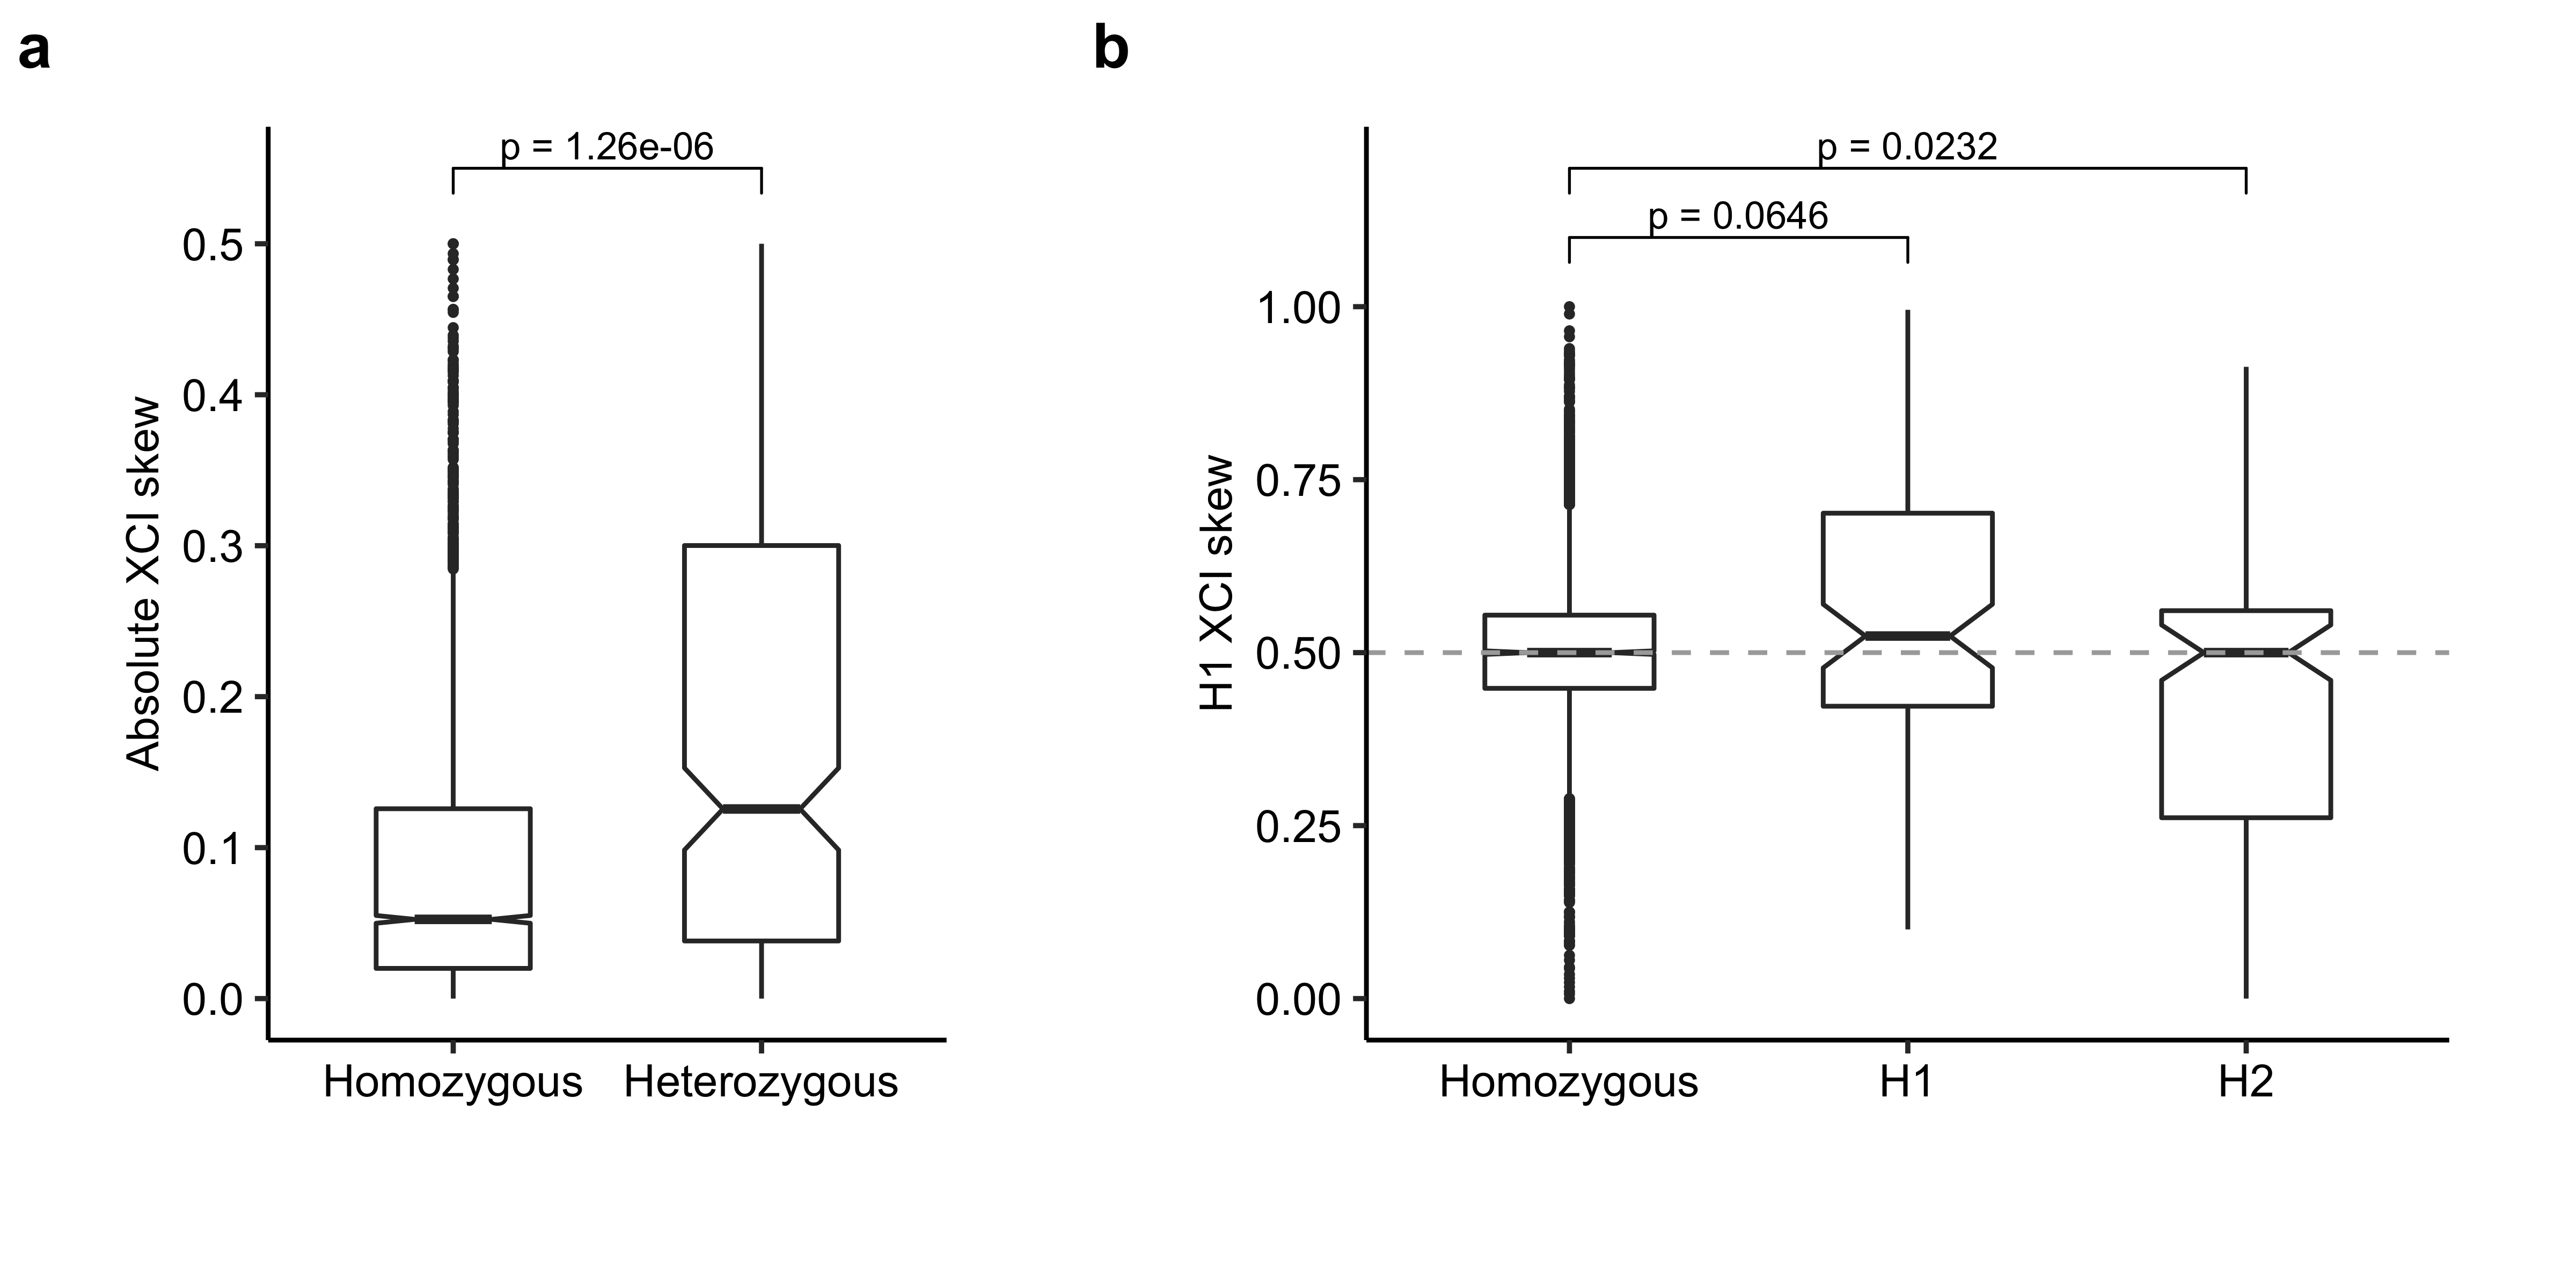
\includegraphics[width=0.9\textwidth]{chapter4/Figures/Supplementary_Figure_4.png}
    \caption{
        Association of LOC101928359 variant (rs73227260) with XCI skew. Indicated p-values are from a linear mixed model accounting for individual and tissue of origin.
        \textbf{a}, Boxplot of absolute XCI skew in homozygous samples (n = 4,230) and heterozygous samples (n = 232). Indicated p-value is from a one-sided t-test.
        \textbf{b}, Boxplot of skewing toward haplotype 1 (H1), where the grouping on the x-axis describes individuals without the LOC variant (Homozygous, n = 4,230), with the variant on haplotype 1 (H1, n = 92), and with the variant on haplotype 2 (H2, n = 140). Indicated p-values are from a two-sided t-test.  
    }
    \label{fig:supp_fig4.4}
\end{figure}